\documentclass[aspectratio=169,xcolor=table]{beamer}
\usepackage[utf8]{inputenc}
\usepackage[T1,T5]{fontenc}
\usepackage{amsmath,booktabs,array,graphicx,pifont,tikz}
\usetikzlibrary{arrows.meta,calc,positioning,fit,backgrounds}

\definecolor{Primary}{HTML}{111B88}
\definecolor{Secondary}{HTML}{101659}
\definecolor{Accent}{HTML}{F2A900}
\definecolor{SoftBlue}{HTML}{EAF2F8}
\definecolor{SoftGray}{HTML}{F3F5F7}
\definecolor{TextGray}{HTML}{4D5966}
\definecolor{RiskRed}{HTML}{A23B3B}
\definecolor{GoodGreen}{HTML}{26734D}
\mode<presentation>{\usetheme{Madrid}\usecolortheme{default}\setbeamertemplate{navigation symbols}{}}
\setbeamercolor{structure}{fg=Primary}
\setbeamercolor{frametitle}{fg=white,bg=Primary}
\setbeamercolor{title}{fg=white,bg=Primary}
\setbeamercolor{block title}{fg=white,bg=Primary}
\setbeamercolor{block body}{fg=black,bg=SoftBlue}
\setbeamercolor{block title alerted}{fg=white,bg=Accent!85!black}
\setbeamercolor{block body alerted}{fg=black,bg=Accent!12}
\setbeamercolor{section in head/foot}{fg=white,bg=Primary}
\setbeamercolor{author in head/foot}{fg=white,bg=Secondary}
\setbeamercolor{date in head/foot}{fg=white,bg=Primary}
\setbeamerfont{section in head/foot}{size=\tiny,series=\bfseries}
\setbeamerfont{author in head/foot}{size=\scriptsize}
\setbeamerfont{date in head/foot}{size=\scriptsize,series=\bfseries}
\setbeamerfont{frametitle}{series=\bfseries}
\setbeamerfont{title}{series=\bfseries}
\newcommand{\decklabel}{Catch-up 03/10/2026}
\setbeamertemplate{itemize item}{\color{Secondary}$\blacktriangleright$}
\setbeamertemplate{itemize subitem}{\color{Accent}$\bullet$}
\setbeamertemplate{headline}{\leavevmode\begin{beamercolorbox}[wd=\paperwidth,ht=2.7ex,dp=1.1ex,leftskip=.35cm,rightskip=.35cm]{section in head/foot}\insertsectionnavigationhorizontal{\dimexpr\paperwidth-.70cm\relax}{}{}\end{beamercolorbox}}
\setbeamertemplate{footline}{\leavevmode\hbox{\begin{beamercolorbox}[wd=.55\paperwidth,ht=2.6ex,dp=1ex,leftskip=.35cm,rightskip=.20cm]{section in head/foot}\usebeamerfont{section in head/foot}\insertsectionhead\end{beamercolorbox}\begin{beamercolorbox}[wd=.27\paperwidth,ht=2.6ex,dp=1ex,center]{author in head/foot}\usebeamerfont{author in head/foot}\decklabel\end{beamercolorbox}\begin{beamercolorbox}[wd=.18\paperwidth,ht=2.6ex,dp=1ex,rightskip=.35cm plus1fil]{date in head/foot}\usebeamerfont{date in head/foot}\hfill\insertframenumber\,/\,\inserttotalframenumber\end{beamercolorbox}}}

\newcommand{\hi}[1]{\textcolor{Primary}{\textbf{#1}}}
\newcommand{\bad}[1]{\textcolor{RiskRed}{\textbf{#1}}}
\newcommand{\good}[1]{\textcolor{GoodGreen}{\textbf{#1}}}
\newcommand{\src}[1]{{\tiny\color{TextGray}[Nguồn: #1]}}
\newcommand{\cmark}{\textcolor{GoodGreen}{\ding{51}}}
\newcommand{\xmark}{\textcolor{RiskRed}{\ding{55}}}
\newcommand{\pmark}{\textcolor{Accent!85!black}{\ding{108}}}
\tikzset{
  box/.style={draw=Primary,fill=SoftBlue,rounded corners=2pt,align=center,font=\small,minimum height=0.9cm},
  lgbox/.style={draw=Accent!85!black,fill=Accent!13,rounded corners=2pt,align=center,font=\small,minimum height=0.9cm},
  nbox/.style={draw=TextGray,fill=SoftGray,rounded corners=2pt,align=center,font=\small,minimum height=0.9cm},
  outbox/.style={draw=GoodGreen,fill=GoodGreen!10,rounded corners=2pt,align=center,font=\small\bfseries,minimum height=0.9cm},
  arr/.style={-{Latex[length=2mm]},thick,draw=TextGray},
}

\title{Contextual Biasing cho ASR:\\Benchmark \& Baseline}
\subtitle{Báo cáo tiến độ theo next step buổi họp 17/09 \textbullet\ Mục tiêu Interspeech 2027}
\author{Nhóm Contextual ASR}
\institute{}
\date{03/10/2026}
\setbeamertemplate{title page}{\begin{centering}\vspace*{0.10cm}
\includegraphics[height=1.08cm]{imgs/logo.png}\par\vspace{0.32cm}\begin{beamercolorbox}[sep=0.50em,center,rounded=true]{title}\usebeamerfont{title}\inserttitle\par\vspace{0.14cm}{\small\insertsubtitle\par}\end{beamercolorbox}\vspace{0.42cm}{\usebeamerfont{author}\insertauthor\par}\vspace{0.10cm}{\usebeamerfont{institute}\insertinstitute\par}\vfill{\usebeamerfont{date}\insertdate\par}\end{centering}}

\begin{document}
\begin{frame}[plain]\titlepage\end{frame}

% =====================================================================
\section{Tiến độ}
\begin{frame}{Next step buổi 17/09 $\rightarrow$ đã làm được gì}
\small\renewcommand{\arraystretch}{1.08}
\begin{tabular}{@{}p{4.2cm}p{8.1cm}c@{}}
\toprule
\textbf{Next step} & \textbf{Kết quả} & \\
\midrule
Setup dataset benchmark & LibriSpeech + IS21 bias list (chuẩn so sánh của mảng), 5 điều kiện context & \cmark\\
Domain & Đề xuất \hi{ConEC} (earnings call, giọng thật, context thật); bộ thuhcsi là \bad{tiếng Trung} & \pmark\\
Metric & Scorer IS21 chính thức + chuẩn hoá Whisper + Recall@K; pipeline khớp số model card & \cmark\\
Setup xong rồi ``xem'' & Chạy full 5.559 câu trên RTX 4090: Whisper-turbo xong, Qwen3-ASR phần lớn xong & \pmark\\
Paper không code $\rightarrow$ implement & Đã kiểm 2 paper mục tiêu; tái hiện xong \hi{baseline của Hou25} & \pmark\\
Deadline & Interspeech 2027 --- hạn nộp \hi{09/02/2027} & \cmark\\
\bottomrule
\end{tabular}
\vfill
\begin{beamercolorbox}[sep=0.40em,center,rounded=true]{block body alerted}
\footnotesize Hôm nay: benchmark + metric đã dựng xong, có \textbf{bảng baseline đầu tiên} và \textbf{3 phát hiện} định hướng method.
\end{beamercolorbox}
\end{frame}

% =====================================================================
\section{Bài toán}
\begin{frame}{Bài toán: nhận đúng bias word (tên riêng, từ hiếm)}
\begin{center}
\begin{tikzpicture}[node distance=0.55cm]
\node[nbox,minimum width=1.6cm] (a) {Audio};
\node[box,right=of a,minimum width=2.3cm] (asr) {Qwen3-ASR\\\footnotesize(frozen)};
\node[nbox,right=of asr,minimum width=2.4cm] (h) {Hypothesis +\\\footnotesize posterior $[T\times V]$};
\node[lgbox,right=of h,minimum width=2.8cm] (c) {Bias list\\\footnotesize\textbf{lấy từ đâu?}};
\node[outbox,right=of c,minimum width=1.8cm] (y) {Transcript};
\draw[arr] (a)--(asr); \draw[arr] (asr)--(h); \draw[arr] (h)--(c); \draw[arr] (c)--(y);
\draw[arr,dashed] (c.south) to[bend left=22] node[below,font=\footnotesize]{context / can thiệp decode} (asr.south);
\node[nbox,above=0.45cm of c,font=\footnotesize,minimum height=0.6cm] (r1) {(1) Retrieve từ corpus};
\node[nbox,above=0.12cm of r1,font=\footnotesize,minimum height=0.6cm] (r2) {(2) Generate từ posterior};
\end{tikzpicture}
\end{center}
\vspace{0.1cm}
\begin{columns}[T,onlytextwidth]
\column{0.48\textwidth}
\begin{block}{Literature hiện tại}
\small Bias list \textbf{được cho sẵn} và \textbf{luôn chứa từ đúng}; method chỉ cần \emph{dùng} list.
\end{block}
\column{0.48\textwidth}
\begin{alertblock}{Hướng của nhóm (chưa chốt method)}
\small Bias list \textbf{phải tự dựng}: retrieve từ corpus hoặc sinh từ phân bố xác suất của ASR, rồi rank.
\end{alertblock}
\end{columns}
\end{frame}

\begin{frame}{Hai paper mục tiêu (cùng tầm Interspeech)}
\small\renewcommand{\arraystretch}{1.22}
\begin{tabular}{@{}p{2.6cm}p{4.9cm}p{5.2cm}@{}}
\toprule
& \textbf{Hou25} --- Interspeech 2025 & \textbf{PTC-Bias} --- arXiv 09/2026 \\
\midrule
Ý tưởng & Scorer chọn top-$k$ bias word (TTS audio $\leftrightarrow$ speech) rồi đưa vào prompt & Phoneme posterior + ``temporal competition'' $\rightarrow$ shortlist + sửa sau decode \\
ASR & Whisper-turbo & SLAM-ASR-7B, \hi{Qwen3-ASR} \\
Train? & Có (scorer) & Không train thêm \\
Bias list & \bad{cho sẵn}, $N\le 2000$ & \bad{cho sẵn}, $N\le 2000$ \\
Kết quả & B-WER $-40\%$ (N=100) & B-WER $-23\%$ so với CTC-Filter \\
Code & \xmark{} $\rightarrow$ tự implement & \cmark{} github.com/aizhiqi-work/PTC-Bias \\
\bottomrule
\end{tabular}
\vfill
\begin{beamercolorbox}[sep=0.40em,center,rounded=true]{block body}
\small Cả hai đều chạy trên \hi{LibriSpeech + IS21} $\Rightarrow$ đây là bộ bắt buộc để so sánh trực tiếp.
\end{beamercolorbox}
\vfill\src{Hou et al., Interspeech 2025, pp.~5183--5187; Ai et al., arXiv 2609.28727}
\end{frame}

% =====================================================================
\section{Benchmark}
\begin{frame}{Dataset: chọn gì, loại gì, vì sao}
\small\renewcommand{\arraystretch}{1.2}
\begin{tabular}{@{}p{3.4cm}p{1.6cm}p{1.6cm}p{5.6cm}@{}}
\toprule
\textbf{Bộ} & \textbf{Ngôn ngữ} & \textbf{Speech} & \textbf{Quyết định} \\
\midrule
\hi{LibriSpeech + IS21} & EN & thật & \cmark{} \textbf{Chính} --- 5.559 câu test, kho 209.291 từ hiếm \\
\hi{ConEC} (Earnings-21/22) & EN & thật & \cmark{} \textbf{Domain} --- context thật: slide, press release, người dự \\
ContextASR-Bench & EN/ZH & TTS & \pmark{} Phụ --- có nhãn domain, nhiều entity \\
thuhcsi/Contextual-Biasing & \bad{ZH} & thật & \xmark{} Từ WenetSpeech; lệch ``làm tiếng Anh trước'' \\
ProfASR-Bench & EN & \bad{TTS} & \xmark{} Chỉ tham khảo \\
Contextual Earnings-22 & EN & thật & \xmark{} Chưa public (``upon acceptance'') \\
\bottomrule
\end{tabular}
\vfill\src{fbai-speech/is21\_deep\_bias; github.com/huangruizhe/ConEC; MrSupW/ContextASR-Bench; github.com/thuhcsi/Contextual-Biasing-Dataset}
\end{frame}

\begin{frame}{Protocol: 5 mức context, từ dễ đến thực tế}
\begin{center}
\begin{tikzpicture}[node distance=0.25cm]
\node[outbox,minimum width=2.2cm,text width=2.0cm,font=\footnotesize] (o) {\textbf{Oracle}\\\mdseries chỉ từ đúng};
\node[box,right=of o,minimum width=2.2cm,text width=2.0cm,font=\footnotesize] (n) {\textbf{N=100--2000}\\đúng + nhiễu};
\node[lgbox,right=of n,minimum width=2.2cm,text width=2.0cm,font=\footnotesize] (m) {\textbf{Missing}\\chỉ có nhiễu};
\node[lgbox,right=of m,minimum width=2.2cm,text width=2.0cm,font=\footnotesize] (k) {\textbf{Không list}\\kho 209k từ};
\node[nbox,right=of k,minimum width=2.2cm,text width=2.0cm,font=\footnotesize] (d) {\textbf{Domain}\\ConEC};
\draw[arr] ([yshift=-0.75cm]o.south west) -- node[below,font=\footnotesize]{càng gần thực tế, càng khó} ([yshift=-0.75cm]d.south east);
\draw[thick,draw=Primary] ([yshift=0.25cm]o.north west) -- ([yshift=0.25cm]n.north east) node[midway,above,font=\footnotesize,text=Primary]{Hou25 / PTC-Bias đánh giá ở đây};
\draw[thick,draw=Accent!85!black] ([yshift=0.25cm]m.north west) -- ([yshift=0.25cm]d.north east) node[midway,above,font=\footnotesize,text=Accent!70!black]{\textbf{chưa ai đánh giá}};
\end{tikzpicture}
\end{center}
\vspace{0.1cm}
\begin{block}{Kiểm tra trên file IS21 gốc}
\small Với mọi câu, list N luôn chứa \textbf{toàn bộ} từ hiếm của reference (vd.\ \texttt{237-134493-0004}: ``intermingled'', ``mated'' đều có trong list 102 từ). Bài toán ``chọn'' dễ hơn bài toán ``tìm'' rất nhiều.
\end{block}
\end{frame}

\begin{frame}{Metric và kiểm chứng pipeline}
\begin{columns}[T,onlytextwidth]
\column{0.50\textwidth}
\begin{block}{Metric}
\small
\begin{itemize}\itemsep3pt
\item \textbf{WER / U-WER / B-WER} --- scorer IS21 chính thức (sub=4, ins/del=3); B-WER tính trên từ hiếm của reference.
\item \textbf{Recall@K, MRR} --- đo riêng bước tạo candidate.
\item Chuẩn hoá: EnglishTextNormalizer (Whisper) cho cả ref, hyp, bias.
\end{itemize}
\end{block}
\column{0.46\textwidth}
\begin{alertblock}{Chuẩn hoá ảnh hưởng lớn}
\small Ref ``in \textbf{honour} of \textbf{saint} francis'' -- Hyp ``in \textbf{honor} of \textbf{st} francis'' $\Rightarrow$ 2 lỗi giả.\\[2pt]
Lệch B-WER $\approx$ \bad{0.5--1 điểm} $\Rightarrow$ paper phải ghi rõ normalizer.
\end{alertblock}
\end{columns}
\vspace{0.25cm}
\begin{center}
\begin{tikzpicture}
\node[outbox,minimum width=11.5cm,font=\normalsize] {Qwen3-ASR, không context, test-clean: WER \textbf{1.63\%} \;=\; model card chính thức \textbf{1.63\%} \;\cmark};
\end{tikzpicture}
\end{center}
\end{frame}

% =====================================================================
\section{Kết quả}
\begin{frame}{Tái hiện Hou25 --- Whisper-large-v3-turbo + prompt}
\small\renewcommand{\arraystretch}{1.25}
\begin{center}
\begin{tabular}{@{}lcccc@{}}
\toprule
& \multicolumn{2}{c}{\textbf{WER} (clean / other)} & \multicolumn{2}{c}{\textbf{B-WER} (clean / other)}\\
\cmidrule(lr){2-3}\cmidrule(lr){4-5}
\textbf{Điều kiện} & Hou25 & \hi{Nhóm chạy} & Hou25 & \hi{Nhóm chạy}\\
\midrule
Không prompt & 3.2 / 5.3 & 2.64 / 4.87 & 10.4 / 19.7 & 9.43 / 18.92\\
+ prompt N=100 & 2.7 / 4.8 & 2.55 / 4.20 & 7.8 / 15.2 & 8.04 / 13.98\\
+ prompt N=2000 & 2.9 / 5.2 & 2.79 / 4.97 & 9.8 / 19.5 & 9.15 / 18.69\\
\bottomrule
\end{tabular}
\end{center}
\vspace{0.15cm}
\begin{columns}[T,onlytextwidth]
\column{0.48\textwidth}
\begin{block}{Khớp}
\small Cùng xu hướng: N=100 giúp; N=2000 \textbf{gần như mất tác dụng} (bias bị loãng).
\end{block}
\column{0.48\textwidth}
\begin{alertblock}{Lệch nhẹ}
\small Số tuyệt đối thấp hơn 0.2--1.2 điểm: Hou25 không nêu normalizer / cấu hình decode. Prompt dài cắt còn 223 token cuối.
\end{alertblock}
\end{columns}
\vfill\src{Hou et al., Interspeech 2025, Bảng 1; full test-clean 2620 + test-other 2939 câu, chuẩn hoá ``plain''}
\end{frame}

\begin{frame}{Qwen3-ASR-1.7B: list càng dài, bias càng mất tác dụng}
\begin{columns}[c,onlytextwidth]
\column{0.52\textwidth}
\begin{center}
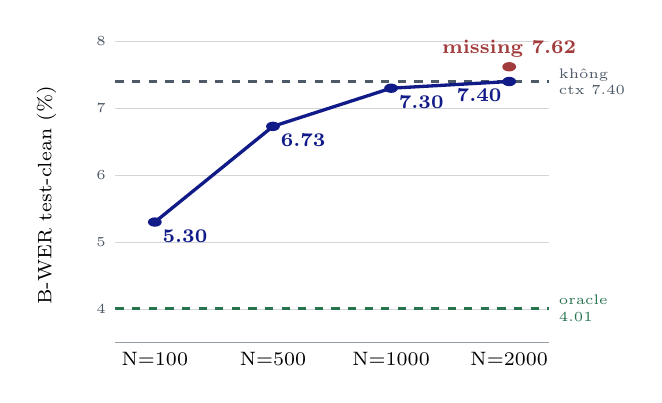
\begin{tikzpicture}[x=1.25cm,y=0.85cm]
% trục y từ 3.5 đến 8
\foreach \y in {4,5,6,7,8}{\draw[TextGray!25] (0,\y-3.5)--(4.4,\y-3.5); \node[left,font=\tiny,TextGray] at (0,\y-3.5){\y};}
\draw[TextGray!60] (0,0)--(4.4,0);
% mức không context và oracle
\draw[TextGray,dashed,thick] (0,7.40-3.5)--(4.4,7.40-3.5) node[right,font=\tiny,text=TextGray,align=left]{không\\ctx 7.40};
\draw[GoodGreen,dashed,thick] (0,4.01-3.5)--(4.4,4.01-3.5) node[right,font=\tiny,text=GoodGreen,align=left]{oracle\\4.01};
% đường B-WER theo N
\draw[Primary,very thick] (0.4,5.30-3.5)--(1.6,6.73-3.5)--(2.8,7.30-3.5)--(4.0,7.40-3.5);
\foreach \x/\v/\l/\p in {0.4/5.30/100/below right, 1.6/6.73/500/below right, 2.8/7.30/1000/below right, 4.0/7.40/2000/below left}{
  \fill[Primary] (\x,\v-3.5) circle (0.07);
  \node[\p=-1pt,font=\scriptsize\bfseries,text=Primary] at (\x,\v-3.5){\v};
  \node[below,font=\scriptsize] at (\x,0){N=\l};
}
\fill[RiskRed] (4.0,7.62-3.5) circle (0.07) node[above,font=\scriptsize\bfseries,text=RiskRed]{missing 7.62};
\node[rotate=90,font=\scriptsize] at (-0.7,2.2){B-WER test-clean (\%)};
\end{tikzpicture}
\end{center}
\column{0.46\textwidth}
\footnotesize\renewcommand{\arraystretch}{1.12}
\begin{tabular}{@{}lccc@{}}
\toprule
\textbf{test-clean} & \textbf{WER} & \textbf{U-WER} & \textbf{B-WER}\\
\midrule
Không context & 1.63 & 0.89 & 7.40\\
Oracle & 1.22 & 0.87 & \good{4.01}\\
N=100 & 1.42 & 0.93 & 5.30\\
N=500 & 1.60 & 0.94 & 6.73\\
N=1000 & 1.67 & 0.95 & 7.30\\
N=2000 & 1.69 & 0.96 & \bad{7.40}\\
Missing N100 & 1.73 & 0.98 & \bad{7.62}\\
\midrule
\multicolumn{4}{@{}l}{test-other: none 16.08 · N100 11.61 · oracle 7.73}\\
\multicolumn{4}{@{}l}{PTC-Bias (N=2000): 4.10 / 7.76}\\
\bottomrule
\end{tabular}
\end{columns}
\vfill\src{Context đưa vào system prompt ``w1, w2, …''; chuẩn hoá Whisper; full test-clean 2620 câu; test-other N500--N2000 đang chạy}
\end{frame}

\begin{frame}{Ba phát hiện định hướng method}
\begin{columns}[T,onlytextwidth]
\column{0.32\textwidth}
\begin{block}{1. List luôn có đáp án}
\small Setting IS21 / Hou25 / PTC-Bias giả định list \textbf{chứa từ đúng}. Thực tế phải \emph{tự tìm} --- chưa ai đo.
\end{block}
\column{0.32\textwidth}
\begin{alertblock}{2. List dài = vô dụng}
\small Qwen3-ASR: B-WER 5.30 $\rightarrow$ 7.40 khi N 100 $\rightarrow$ 2000, tức \textbf{bằng không context}; list sai còn tệ hơn (\bad{7.62}). Oracle 4.01 $\Rightarrow$ phần ``chọn đúng candidate'' phải lấy lại.
\end{alertblock}
\column{0.32\textwidth}
\begin{block}{3. Normalizer quan trọng}
\small Lệch 0.5--1 điểm B-WER chỉ do chuẩn hoá $\Rightarrow$ mọi so sánh phải cùng pipeline (đã tự chạy lại baseline).
\end{block}
\end{columns}
\vspace{0.3cm}
\begin{beamercolorbox}[sep=0.45em,center,rounded=true]{block body alerted}
\small Câu hỏi nghiên cứu nổi lên: \textbf{khi không có list cho sẵn, làm sao dựng được list ngắn mà vẫn chứa từ đúng?}\\
$\rightarrow$ đúng hai hướng của buổi 17/09: retrieve từ corpus / generate từ posterior + ranking.
\end{beamercolorbox}
\end{frame}

% =====================================================================
\section{Kế hoạch}
\begin{frame}{Kế hoạch tới hạn Interspeech 2027 (09/02/2027)}
\begin{center}
\begin{tikzpicture}[x=1.3cm]
\draw[arr,very thick] (0,0)--(10.4,0);
\foreach \x/\pa/\pb/\pc in {
 0.4/{10}/{Tái hiện method}/{PTC-Bias (code)\\Hou25 (tự viết)},
 2.6/{11}/{Setting khó}/{missing / không list\\ConEC},
 4.8/{11--12}/{Method}/{retrieve vs generate\\+ ranking},
 7.0/{12--01}/{Ablation}/{phân tích lỗi\\over-biasing},
 9.2/{01--02}/{Viết \& nộp}/{4 trang\\09/02/2027}}{
  \fill[Primary] (\x,0) circle (0.11);
  \node[above=0.15cm,font=\footnotesize\bfseries,text=Primary,align=center] at (\x,0){Tháng \pa\\\pb};
  \node[below=0.2cm,font=\scriptsize,align=center,text=TextGray] at (\x,0){\pc};
}
\end{tikzpicture}
\end{center}
\vspace{0.15cm}
\begin{columns}[T,onlytextwidth]
\column{0.48\textwidth}
\begin{block}{Việc ngay sau buổi họp}
\small
\begin{itemize}\itemsep2pt
\item Chạy xong Qwen3-ASR: N500/N1000/N2000, missing.
\item Chạy method PTC-Bias trên pipeline của nhóm.
\item Implement scorer Hou25; tải ConEC.
\end{itemize}
\end{block}
\column{0.48\textwidth}
\begin{alertblock}{Mốc kiểm soát}
\small \textbf{Cuối tháng 11}: số của PTC-Bias/Hou25 ở setting khó. Sụt mạnh $\Rightarrow$ có motivation; nếu không $\Rightarrow$ đổi trục.
\end{alertblock}
\end{columns}
\end{frame}

\begin{frame}{Cần thầy quyết để đi tiếp}
\renewcommand{\arraystretch}{1.3}
\begin{tabular}{@{}cp{7.2cm}p{4.6cm}@{}}
\toprule
& \textbf{Câu hỏi} & \textbf{Đề xuất của nhóm}\\
\midrule
\hi{1} & Thay bộ thuhcsi (tiếng Trung) bằng \textbf{ConEC} làm bộ domain? & Đồng ý ConEC; thuhcsi để dành nếu mở sang tiếng Trung\\
\hi{2} & Được dùng \textbf{GPU server} lâu dài? (PTC-Bias, Hou25 cần train module nhỏ) & 1$\times$RTX 4090 là đủ\\
\hi{3} & Chốt method \textbf{bây giờ} hay \textbf{sau khi} có số baseline ở setting khó? & Sau --- cuối tháng 10\\
\hi{4} & Ưu tiên hướng nào: \textbf{retrieve từ corpus} hay \textbf{generate từ posterior}? & Thử cả hai ở mức Recall@K trước\\
\hi{5} & ``Can thiệp ảo'' model: chỉ context/logit, hay cả hidden state? & Context + logit (model frozen)\\
\bottomrule
\end{tabular}
\end{frame}

\begin{frame}{Tóm tắt}
\begin{center}
\begin{tikzpicture}[node distance=0.35cm,minimum height=1.5cm]
\node[outbox,minimum width=3.4cm,text width=3.2cm] (a) {Benchmark + metric\\\mdseries\footnotesize đã dựng, đã kiểm chứng};
\node[outbox,right=of a,minimum width=3.4cm,text width=3.2cm] (b) {Baseline Hou25\\\mdseries\footnotesize tái hiện đúng xu hướng};
\node[lgbox,right=of b,minimum width=3.4cm,text width=3.2cm] (c) {\textbf{Gap}\\\footnotesize list cho sẵn $\ne$ thực tế};
\draw[arr] (a)--(b); \draw[arr] (b)--(c);
\end{tikzpicture}
\end{center}
\vspace{0.3cm}
\begin{beamercolorbox}[sep=0.55em,center,rounded=true]{block body alerted}
Benchmark đã dựng, baseline đã tái hiện và pipeline khớp số chính thức.\\
Các method hiện tại đều giả định list có sẵn từ đúng $\rightarrow$ bước tiếp: đo chúng sụt bao nhiêu khi bỏ giả định đó.
\end{beamercolorbox}
\end{frame}

% =====================================================================
\section{Phụ lục}
\begin{frame}{Phụ lục: setup chạy thực nghiệm}
\small
\begin{columns}[T,onlytextwidth]
\column{0.48\textwidth}
\begin{block}{Cấu hình}
\begin{itemize}\itemsep2pt
\item 1$\times$RTX 4090, image \texttt{nvcr.io/nvidia/pytorch:26.08}.
\item Whisper-large-v3-turbo (HF, greedy), prompt ``naive''.
\item Qwen3-ASR-1.7B (\texttt{qwen-asr} 0.0.6), \texttt{context} = system prompt.
\item Code: \texttt{bench/} (build\_is21, run\_*, score, eval\_retrieval).
\end{itemize}
\end{block}
\column{0.48\textwidth}
\begin{block}{Whisper-turbo, chuẩn hoá Whisper}
\renewcommand{\arraystretch}{1.15}
\begin{tabular}{@{}lcc@{}}
\toprule
& WER & B-WER\\
\midrule
không prompt & 2.17 / 4.25 & 8.67 / 17.90\\
N=100 & 2.07 / 3.64 & 7.27 / 13.48\\
N=2000 & 2.32 / 4.39 & 8.34 / 17.83\\
\bottomrule
\end{tabular}
\end{block}
\end{columns}
\end{frame}

\end{document}
